
\documentclass[conference]{IEEEtran}

\IEEEoverridecommandlockouts

\usepackage{cite}
\usepackage{amsmath,amssymb,amsfonts}
\usepackage{algorithmic}
\usepackage{graphicx}
\graphicspath{{figures/}}
\usepackage{textcomp}
\usepackage{xcolor}
\usepackage{booktabs}
\usepackage{multirow}
\usepackage{array}
\usepackage{url}
\usepackage{hyperref}
\usepackage{float}

\def\BibTeX{{\rm B\kern-.05em{\sc i\kern-.025em b}\kern-.08em
T\kern-.1667em\lower.7ex\hbox{E}\kern-.125emX}}

\begin{document}

\title{Logos: A Resource-Aware Experimental Framework for Efficient Decoder-Only Language Models}

\author{
\IEEEauthorblockN{Spandan Basu Chaudhuri}
\IEEEauthorblockA{
Department of Computer Science and Engineering\\
SRM Institute of Science and Technology\\
Chennai, India\\
Email: spandanbasu139@gmail.com
}
}

\maketitle

\begin{abstract}
Decoder-only language models have become the dominant architecture for modern generative artificial intelligence, but their practical deployment is constrained by parameter count, checkpoint size, memory consumption, inference latency, throughput, and hardware cost. This paper presents \textit{Logos}, a resource-aware experimental framework for studying efficient decoder-only language models under controlled training and deployment conditions. Instead of treating perplexity as the only indicator of model quality, Logos evaluates models through a broader efficiency-oriented lens that includes parameter count, validation loss, perplexity, checkpoint size, peak VRAM usage, inference latency, and deployment feasibility. The current experimental cycle begins with preliminary Experiments 1--10, where the basic GPT-style training pipeline, dataset preparation, tokenizer flow, loss tracking, validation loop, and early decoder-only configurations were developed. The later documented sequence begins with a 32.16M-parameter GPT-style baseline and progressively introduces weight tying, SwiGLU feed-forward layers, wider-shallower compact scaling, medium and large model scaling, longer training schedules, and FP16 compression. The best trained model, Exp18, uses 124.03M parameters and reaches a perplexity of 53.57 after 15,000 iterations on an OpenWebText subset with context length 512. The deployment-oriented Exp19 reduces checkpoint size from 473.20 MB to 310.24 MB and lowers peak inference VRAM to approximately 5.96 GB. Experiments were conducted using a workstation equipped with an NVIDIA RTX 6000 Ada 48 GB GPU, which enabled controlled training and evaluation without requiring large-scale distributed infrastructure. The paper also proposes a preliminary Logos Efficiency Index and argues that separate efficiency leaderboards are more reliable than a single universal score. Current results show that simple architectural, training, and deployment choices can significantly improve capability per resource, while also identifying the need for stronger architecture-level novelty in future Logos versions.
\end{abstract}

\begin{IEEEkeywords}
Language models, decoder-only Transformer, efficient language modeling, SwiGLU, weight tying, model compression, perplexity, resource-aware AI, compact LLMs.
\end{IEEEkeywords}

\section{Introduction}

Decoder-only Transformer language models have become the foundation of modern text generation, code generation, reasoning assistance, and conversational artificial intelligence. However, the rapid scaling of these models has created a major research and engineering challenge: stronger models often require larger parameter counts, larger datasets, longer training schedules, greater memory capacity, higher inference cost, and more specialized hardware. While very large models remain important, there is also a practical need to understand how much capability can be obtained from smaller and more efficient decoder-only models.

The Logos project addresses this problem from a resource-aware experimental perspective. Instead of focusing only on the lowest possible perplexity, Logos studies how model quality changes with parameter count, architecture choices, training duration, context length, checkpoint size, VRAM consumption, inference cost, and deployment feasibility. This allows model variants to be compared not only as language models, but also as deployable systems.

The central idea behind Logos is that efficient language modeling should be evaluated as a trade-off problem. A model with the lowest perplexity is not always the most practical model. For example, a model may achieve better validation loss but require substantially more GPU memory, larger checkpoint storage, or slower token generation. In contrast, a slightly weaker model may be more useful if it can be trained, stored, and deployed on a single workstation GPU. This distinction is especially important for independent researchers, academic projects, and hardware-constrained development environments.

The current Logos cycle investigates a sequence of controlled experiments. Experiments 1--10 represent the preliminary development phase, where the core training code, dataset handling, model skeleton, validation logic, and early architectural decisions were built and tested. The later documented experimental ladder begins with a 32.16M-parameter GPT-style decoder-only baseline model trained on an OpenWebText subset. Subsequent experiments introduce weight tying, SwiGLU feed-forward networks, compact wider-shallower design, medium and large scaling, longer training schedules, and FP16 deployment compression. The best trained model so far is Exp18, a 124.03M-parameter decoder-only model trained for 15,000 iterations, achieving a perplexity of 53.57. A compressed deployment version, Exp19, reduces checkpoint size and VRAM usage while maintaining practical inference feasibility.

All experiments in the current cycle were designed around practical hardware availability. The main training and evaluation environment used an NVIDIA RTX 6000 Ada 48 GB GPU. This hardware setting is important because it represents a powerful but still single-GPU research workstation configuration, rather than a large distributed cluster. Therefore, Logos is positioned as a controlled efficiency study that can be repeated, extended, and compared under realistic academic and workstation-level constraints.

The current contribution should be framed carefully. Logos is not yet a new Transformer architecture, a new optimization algorithm, or a patent-level invention. Its present contribution is a structured resource-aware experimental framework for efficient decoder-only language modeling. The project provides a controlled experimental ladder, empirical observations on scaling and compression, and a foundation for future architecture-level novelty.

\begin{figure}[H]
    \centering
    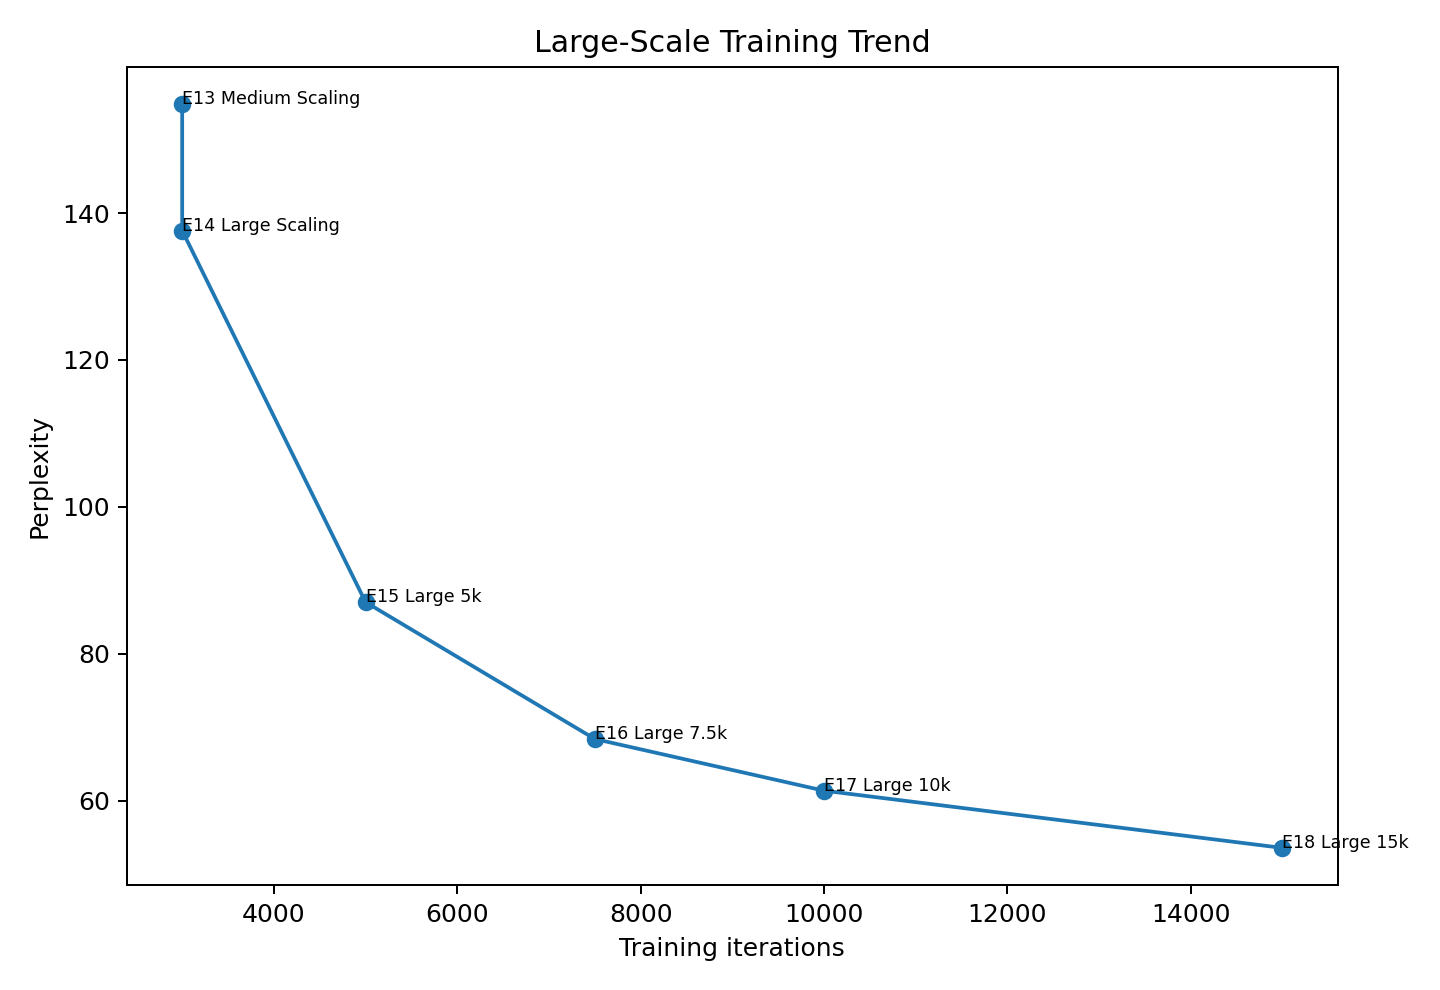
\includegraphics[width=0.95\linewidth]{large_training_trend.png}
    \caption{Corrected-report training and perplexity trend for the major Logos experiments.}
    \label{fig:ppl_trend}
\end{figure}

\begin{figure}[H]
    \centering
    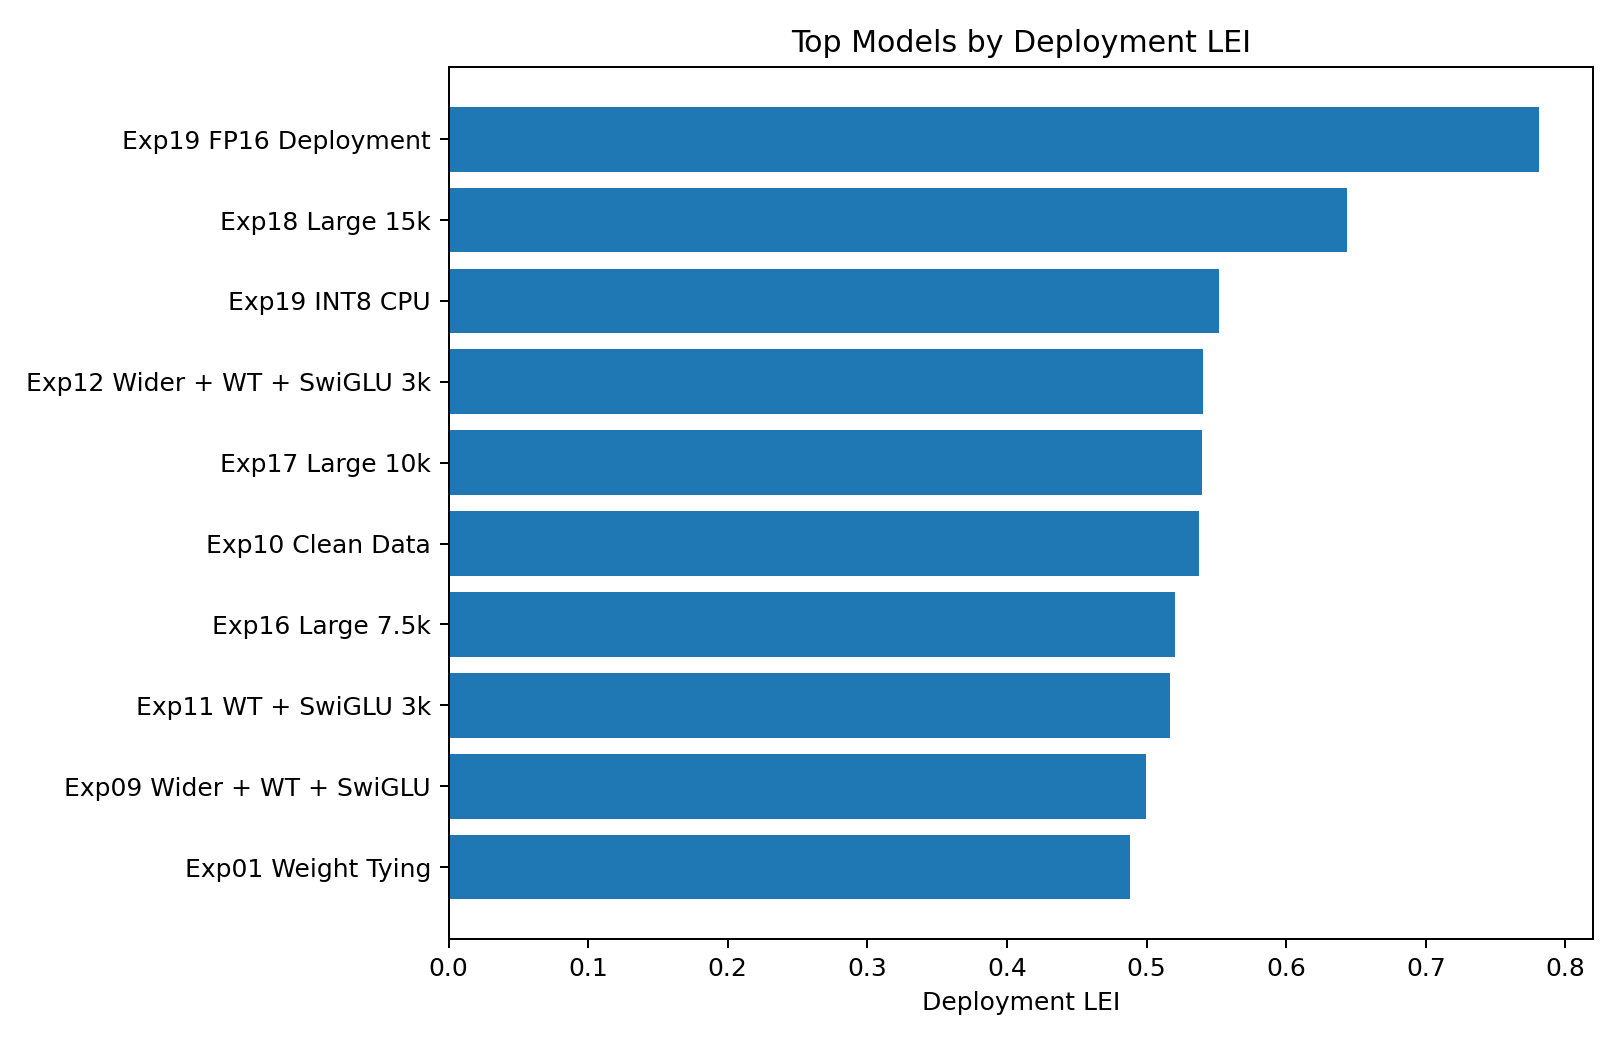
\includegraphics[width=0.95\linewidth]{deployment_lei_top10.png}
    \caption{Corrected-report deployment-oriented Logos Efficiency Index ranking.}
    \label{fig:deployment_lei}
\end{figure}

\begin{figure}[H]
    \centering
    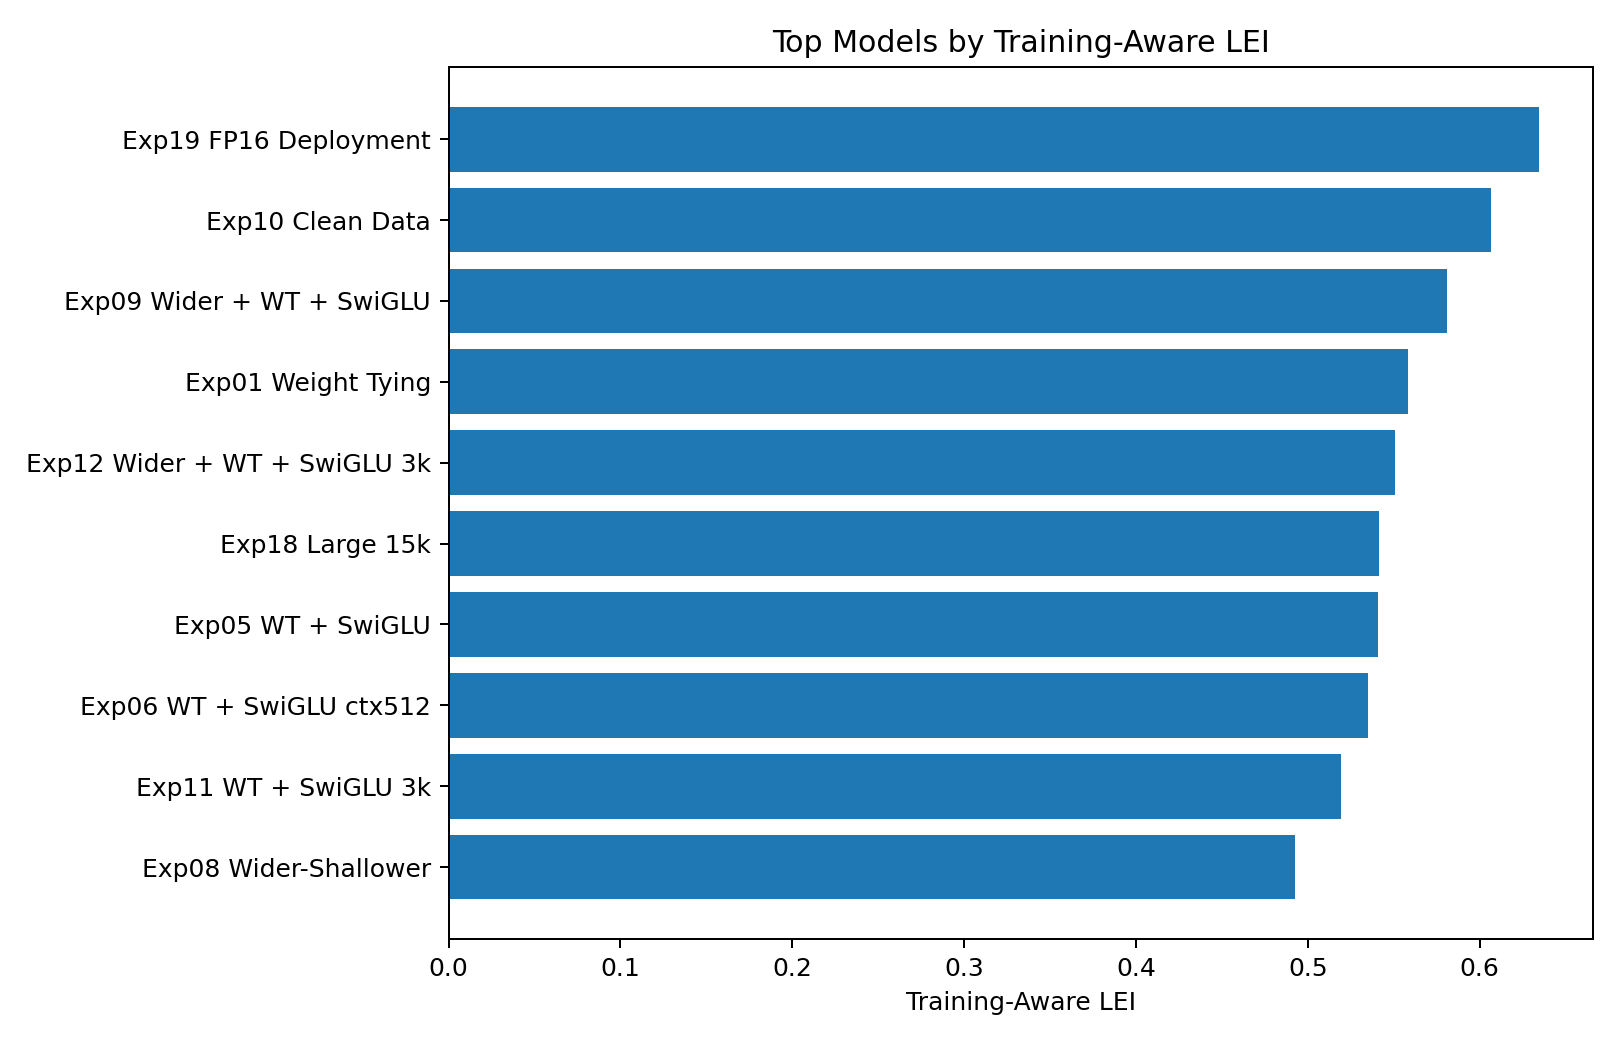
\includegraphics[width=0.95\linewidth]{training_aware_lei_top10.png}
    \caption{Corrected-report training-aware Logos Efficiency Index ranking.}
    \label{fig:training_aware_lei}
\end{figure}

\subsection{Interpretation of Internal Baselines}

The internal Logos ladder provides three important anchors for future work. Exp12 is the compact-efficiency anchor because it has the smallest parameter count among the strong compact models. Exp18 is the quality anchor because it achieves the best perplexity. Exp19 is the deployment anchor because it provides the most practical compressed version.

Any future Logos 0.6 architecture experiment should compare against all three anchors. If a new architecture improves perplexity but greatly increases VRAM or latency, it may not be a true efficiency improvement. Similarly, if it reduces memory but damages perplexity too much, it may not be useful. The aim should be to improve the Pareto frontier between quality and resource cost.

\section{Limitations}

The current work has several limitations.

First, the model is still based on a standard decoder-only Transformer. Therefore, the project should not claim architecture-level novelty yet.

Second, the training data size is much smaller than the datasets used by many public pretrained models. Direct comparison with models such as GPT-2, Pythia, and SmolLM2 must acknowledge differences in dataset size, tokenizer, training tokens, and compute budget.

Third, current evaluation is mainly based on perplexity and system metrics. More downstream benchmarks are needed to understand reasoning, factuality, code ability, and instruction-following performance.

Fourth, the Logos Efficiency Index is still preliminary. It is useful as an exploratory metric, but the project currently treats separate leaderboards as more reliable.

Fifth, the current paper still needs final figures, an architecture diagram, hardware setup details, and a stronger related work section before submission.


\section{Remaining Diagram Placeholders}

The following figures are intentionally kept as placeholders because they should be created as clean diagrams rather than extracted result charts.

\begin{figure}[H]
    \centering
    \fbox{\parbox{0.92\linewidth}{
    \centering
    \vspace{1.2cm}
    \textbf{Placeholder: Logos Experimental Pipeline Diagram}\\
    Show OpenWebText input, preprocessing, Exp1--Exp10 setup, Exp11--Exp12 compact models, Exp13--Exp18 scaling, Exp19 compression, and Exp20 efficiency analysis.
    \vspace{1.2cm}
    }}
    \caption{Placeholder for the overall Logos experimental pipeline.}
    \label{fig:placeholder_pipeline}
\end{figure}

\begin{figure}[H]
    \centering
    \fbox{\parbox{0.92\linewidth}{
    \centering
    \vspace{1.2cm}
    \textbf{Placeholder: Logos Decoder-Only Architecture Diagram}\\
    Show token embedding, positional embedding, repeated causal Transformer decoder blocks, SwiGLU feed-forward network, residual connections, layer normalization, and weight-tied LM head.
    \vspace{1.2cm}
    }}
    \caption{Placeholder for the current Logos architecture diagram.}
    \label{fig:placeholder_architecture}
\end{figure}

\begin{figure}[H]
    \centering
    \fbox{\parbox{0.92\linewidth}{
    \centering
    \vspace{1.2cm}
    \textbf{Placeholder: Dataset and Training Workflow Diagram}\\
    Show OpenWebText samples, tokenization, token IDs, context windows, train-validation split, training loop, validation loss, and perplexity calculation.
    \vspace{1.2cm}
    }}
    \caption{Placeholder for the dataset and training workflow diagram.}
    \label{fig:placeholder_dataset_workflow}
\end{figure}

\begin{figure}[H]
    \centering
    \fbox{\parbox{0.92\linewidth}{
    \centering
    \vspace{1.2cm}
    \textbf{Placeholder: Logos 0.6 Future Roadmap}\\
    Show future architecture ideation directions such as better attention, hybrid local-global attention, efficient FFN redesign, adaptive context, memory modules, early exit, token-importance computation, and better efficiency metrics.
    \vspace{1.2cm}
    }}
    \caption{Placeholder for the Logos 0.6 future architecture roadmap.}
    \label{fig:placeholder_future_roadmap}
\end{figure}

\section{Future Work}

The immediate next experimental direction is context-length scaling. The planned Exp21 or Exp22 tests the 124M model with context length 1024, batch size 16, 100k OpenWebText samples, and an initial training budget of 3000 iterations. On the NVIDIA RTX 6000 Ada 48 GB GPU, this experiment is expected to fit within memory, likely using approximately 25--35 GB VRAM depending on implementation and batch configuration.

The goal of the context-length experiment is to test whether increasing the context window from 512 to 1024 provides measurable improvement. Longer context allows the model to condition on more previous tokens, which may improve long-range dependency modeling. However, longer context also increases attention memory and compute cost. This makes the experiment useful for evaluating the trade-off between context capacity and resource usage.

The broader future direction is Logos 0.6, which may move from resource-aware benchmarking toward architecture-level novelty. Potential directions include:

\begin{itemize}
    \item improved attention mechanisms,
    \item hybrid local-global attention,
    \item parameter-efficient feed-forward redesign,
    \item adaptive context usage,
    \item lightweight memory modules,
    \item token-importance-based computation,
    \item dynamic depth or early-exit inference,
    \item improved efficiency metrics beyond LEI.
\end{itemize}

The current goal is not to replace the architecture immediately, but to study which architectural modifications are likely to improve capability per parameter, checkpoint size, VRAM, latency, throughput, and watt efficiency.

\begin{figure}[H]
    \centering
    \fbox{\parbox{0.92\linewidth}{
    \centering
    \vspace{1.2cm}
    \textbf{Placeholder for Figure 6}\\
    Future Logos 0.6 architecture exploration map: attention redesign, FFN redesign, adaptive context, memory module, early exit, and efficiency metric extension.
    \vspace{1.2cm}
    }}
    \caption{Placeholder for the Logos 0.6 future architecture planning diagram.}
    \label{fig:future_architecture}
\end{figure}

\section{Conclusion}

This paper presents the current state of Logos, a resource-aware experimental framework for efficient decoder-only language models. The project begins with a 32.16M-parameter GPT-style baseline and progressively explores architectural efficiency, compact design, scaling, longer training, compression, and efficiency ranking. The strongest trained model, Exp18, reaches a perplexity of 53.57 with 124.03M parameters after 15,000 iterations. The compressed deployment model, Exp19, reduces checkpoint size to 310.24 MB and peak inference VRAM to approximately 5.96 GB. 

The main conclusion is that efficient language modeling requires evaluating both capability and resource cost. Logos currently provides a strong controlled framework for such evaluation, while future work should focus on architecture-level changes that can create stronger research novelty.

\section*{Acknowledgment}

The author expresses sincere gratitude to Prof. Nagamalleshwari for her guidance, support, and academic supervision throughout the development of this work. The author also acknowledges SRM Institute of Science and Technology for providing an academic environment that supported this research-oriented project. The experiments were carried out using a workstation equipped with an NVIDIA RTX 6000 Ada 48 GB GPU, which enabled controlled single-GPU training, evaluation, and deployment analysis. The author also acknowledges the open-source research community and the availability of open datasets and machine learning tools that made this experimental study possible.

\begin{thebibliography}{00}{00}

\bibitem{vaswani2017attention}
A. Vaswani et al., ``Attention is All You Need,'' in \textit{Advances in Neural Information Processing Systems}, 2017.

\bibitem{radford2019language}
A. Radford et al., ``Language Models are Unsupervised Multitask Learners,'' OpenAI, 2019.

\bibitem{brown2020language}
T. Brown et al., ``Language Models are Few-Shot Learners,'' in \textit{Advances in Neural Information Processing Systems}, 2020.

\bibitem{shazeer2020glu}
N. Shazeer, ``GLU Variants Improve Transformer,'' arXiv preprint arXiv:2002.05202, 2020.

\bibitem{press2017using}
O. Press and L. Wolf, ``Using the Output Embedding to Improve Language Models,'' in \textit{Proceedings of EACL}, 2017.

\bibitem{biderman2023pythia}
S. Biderman et al., ``Pythia: A Suite for Analyzing Large Language Models Across Training and Scaling,'' in \textit{Proceedings of ICML}, 2023.

\bibitem{touvron2023llama}
H. Touvron et al., ``LLaMA: Open and Efficient Foundation Language Models,'' arXiv preprint arXiv:2302.13971, 2023.

\bibitem{dao2022flashattention}
T. Dao et al., ``FlashAttention: Fast and Memory-Efficient Exact Attention with IO-Awareness,'' in \textit{Advances in Neural Information Processing Systems}, 2022.

\bibitem{dettmers2022llmint8}
T. Dettmers et al., ``LLM.int8(): 8-bit Matrix Multiplication for Transformers at Scale,'' in \textit{Advances in Neural Information Processing Systems}, 2022.

\bibitem{openwebtext}
A. Gokaslan and V. Cohen, ``OpenWebText Corpus,'' 2019. [Online]. Available: \url{https://skylion007.github.io/OpenWebTextCorpus/}

\bibitem{devlin2019bert}
J. Devlin, M.-W. Chang, K. Lee, and K. Toutanova, ``BERT: Pre-training of Deep Bidirectional Transformers for Language Understanding,'' in \textit{Proceedings of NAACL-HLT}, 2019.

\bibitem{raffel2020t5}
C. Raffel et al., ``Exploring the Limits of Transfer Learning with a Unified Text-to-Text Transformer,'' \textit{Journal of Machine Learning Research}, vol. 21, no. 140, pp. 1--67, 2020.

\bibitem{kaplan2020scaling}
J. Kaplan et al., ``Scaling Laws for Neural Language Models,'' arXiv preprint arXiv:2001.08361, 2020.

\bibitem{hoffmann2022training}
J. Hoffmann et al., ``Training Compute-Optimal Large Language Models,'' arXiv preprint arXiv:2203.15556, 2022.

\bibitem{su2021roformer}
J. Su, Y. Lu, S. Pan, B. Wen, and Y. Liu, ``RoFormer: Enhanced Transformer with Rotary Position Embedding,'' arXiv preprint arXiv:2104.09864, 2021.

\bibitem{ba2016layer}
J. L. Ba, J. R. Kiros, and G. E. Hinton, ``Layer Normalization,'' arXiv preprint arXiv:1607.06450, 2016.

\bibitem{hendrycks2016gelu}
D. Hendrycks and K. Gimpel, ``Gaussian Error Linear Units (GELUs),'' arXiv preprint arXiv:1606.08415, 2016.

\bibitem{micikevicius2018mixed}
P. Micikevicius et al., ``Mixed Precision Training,'' in \textit{Proceedings of ICLR}, 2018.

\bibitem{hu2022lora}
E. J. Hu et al., ``LoRA: Low-Rank Adaptation of Large Language Models,'' in \textit{Proceedings of ICLR}, 2022.

\bibitem{frantar2023gptq}
E. Frantar, S. Ashkboos, T. Hoefler, and D. Alistarh, ``GPTQ: Accurate Post-Training Quantization for Generative Pre-trained Transformers,'' in \textit{Proceedings of ICLR}, 2023.


\bibitem{kingma2015adam}
D. P. Kingma and J. Ba, ``Adam: A Method for Stochastic Optimization,'' in \textit{Proceedings of ICLR}, 2015.

\bibitem{loshchilov2019adamw}
I. Loshchilov and F. Hutter, ``Decoupled Weight Decay Regularization,'' in \textit{Proceedings of ICLR}, 2019.

\bibitem{loshchilov2017sgdr}
I. Loshchilov and F. Hutter, ``SGDR: Stochastic Gradient Descent with Warm Restarts,'' in \textit{Proceedings of ICLR}, 2017.

\bibitem{hendrycks2021measuring}
D. Hendrycks et al., ``Measuring Massive Multitask Language Understanding,'' in \textit{Proceedings of ICLR}, 2021.

\bibitem{paperno2016lambada}
D. Paperno et al., ``The LAMBADA Dataset: Word Prediction Requiring a Broad Discourse Context,'' in \textit{Proceedings of ACL}, 2016.

\bibitem{merity2017regularizing}
S. Merity, N. S. Keskar, and R. Socher, ``Regularizing and Optimizing LSTM Language Models,'' in \textit{Proceedings of ICLR}, 2018.

\bibitem{grave2017efficient}
E. Grave, A. Joulin, and N. Usunier, ``Improving Neural Language Models with a Continuous Cache,'' in \textit{Proceedings of ICLR}, 2017.

\bibitem{dai2019transformerxl}
Z. Dai et al., ``Transformer-XL: Attentive Language Models Beyond a Fixed-Length Context,'' in \textit{Proceedings of ACL}, 2019.

\bibitem{kitaev2020reformer}
N. Kitaev, L. Kaiser, and A. Levskaya, ``Reformer: The Efficient Transformer,'' in \textit{Proceedings of ICLR}, 2020.

\bibitem{beltagy2020longformer}
I. Beltagy, M. E. Peters, and A. Cohan, ``Longformer: The Long-Document Transformer,'' arXiv preprint arXiv:2004.05150, 2020.

\bibitem{zaheer2020bigbird}
M. Zaheer et al., ``Big Bird: Transformers for Longer Sequences,'' in \textit{Advances in Neural Information Processing Systems}, 2020.

\bibitem{dao2023flashattention2}
T. Dao, ``FlashAttention-2: Faster Attention with Better Parallelism and Work Partitioning,'' arXiv preprint arXiv:2307.08691, 2023.


\end{thebibliography}

\end{document}
